\documentclass[a4paper,doc,natbib]{apa6}
\usepackage[english]{babel}
\usepackage[utf8x]{inputenc}
\usepackage{amsmath}
\usepackage{graphicx}
\usepackage[colorinlistoftodos]{todonotes}
\usepackage{epstopdf}
\usepackage{url}
\usepackage{mathtools}
\usepackage{csquotes}
\usepackage[hidelinks]{hyperref}
\usepackage{csquotes}
\usepackage{subfigure}
\usepackage{booktabs}
\usepackage[section]{placeins}
\usepackage[sc]{mathpazo}
\usepackage{caption}
\usepackage{authblk}
%\captionsetup[table]{skip=8pt}
\usepackage{placeins}

% ---------- watermark -----------
\usepackage[firstpage]{draftwatermark}
\SetWatermarkAngle{0}
\SetWatermarkFontSize{0.25cm}
\SetWatermarkVerCenter{0.75cm}
\SetWatermarkLightness{0.5}
\SetWatermarkHorCenter{14cm}
\SetWatermarkText{\shortstack[l]{
Navarro, D. J., Tran, P. and Baz, N. (2018). Aversion to option loss in a \\
restless bandit task. Computational Brain and Behavior, 1, 151-164 \\
https://dx.doi.org/10.1007/s42113-018-0010-8
}}
\SetWatermarkScale{1}
% -------------------------------




% comment this line out for manuscript version
\linespread{1.05} % Palatino needs more leading

\affiliation{\hspace*{2pt}} % hack to suppress default text

\title{Aversion to option loss in a restless bandit task}
\shorttitle{Loss aversion with restless bandits}

\author[1]{\normalsize Danielle J. Navarro}
\author[1]{\normalsize Peter Tran}
\author[1]{\normalsize Nicole Baz}


\affil[1]{\small School of Psychology, University of New South Wales, NSW 2052, Australia}

\keywords{Sequential decision making; loss aversion; dynamic environments; reinforcement learning; bandit tasks}

\authornote{This research was supported by Australian Research Discovery Grant DP150104206. Please address all correspondence to Danielle J. Navarro, School of Psychology, University of New South Wales, Sydney, NSW, Australia, 2052. E-mail: d.navarro@unsw.edu.au. Author contributions: project concept (DJN, PT), experiment coding (DJN), data collection (DJN, PT), model implementation and data analysis (DJN), manuscript writing (DJN), literature review (DJN, PT, NB). Data, analysis and experiment code associated with the project are available as an OSF repository at \url{https://osf.io/nzvqp/}}

\abstract{
In everyday life people need to make choices without full information about the environment, which poses an explore-exploit dilemma in which one must balance the need to learn about the world and the need to obtain rewards from it. The explore-exploit dilemma is often studied using the multi-armed restless bandit task, in which people repeatedly select from multiple options, and human behaviour is modelled as a form of reinforcement learning via Kalman filters. Inspired by work in the judgment and decision-making literature, we present two experiments using multi-armed bandit tasks in both static and dynamic environments, in situations where options can become {\it unviable} and vanish if they are not pursued. A Kalman filter model using Thompson sampling provides an excellent account of human learning in a standard restless bandit task, but there are systematic departures in the {\it vanishing bandit} task. We explore the nature of this loss aversion signal and consider theoretical explanations for the results.
}

\begin{document}
\maketitle

\section{Introduction}

In everyday life we make a variety of decisions ranging from simple questions (e.g., what should I have for lunch?) to complex life choices (e.g., should I change jobs?). Often we need to make these choices without full information about what the payoffs will be, and in an environment where the payoff distribution itself can change over time -- some careers might be lucrative today but irrelevant tomorrow -- posing a complex {\it explore-exploit dilemma} for the decision maker \citep{mehlhorn2015unpacking}. The explore exploit trade-off has been studied in a variety of literatures including machine learning \citep{kaelbling1998planning}, statistics \citep{wald1947sequential} and psychology \citep{wilson2014humans}. In the psychological literature these problems are often studied using multi-armed bandit problems, where the decision maker is presented with several possible options that they must repeatedly choose between, and the distribution of rewards associated with each option is unknown to the decision maker \citep[e.g.,][]{banks1997experimental,speekenbrink2015uncertainty, daw2006cortical, steyvers2009bayesian,cohen2007should,zhang2013forgetful,biele2009learning,acuna2010structure,yi2009modeling,anderson2012ambiguity,reverdy2014modeling}. For simpler versions of the multi-armed bandit problem, there are closed form solutions for optimal decisions \citep{whittle1980multi} but in general this is not the case \citep[see][]{burtini2015survey}.

There is a relatively well-established pattern of findings for human performance in this kind of sequential decision task. For instance  people typically show an inherent preference for information \citep{bennett2016intrinsic,navarro2016learning}, though there are a number of learning and decision making problems that show different patterns \citep{iigaya2016modulation,zhu2017information,gigerenzer2017cassandra}. Moreover, the tendency to engage in exploratory behaviour changes systematically: it increases with cognitive capacity \citep{hills2012dynamic}, aspiration level \citep{hausmann2008sequential}, and level of resources \citep{perry2013neural}, decreases with age \citep{mata2013foraging}, and is influenced by prior knowledge about payoff distributions \citep{mulder2012bias} and beliefs about the volatility of the environment \citep{yi2009modeling,navarro2016learning}. Finally, the decision policies that human and machine agents employ typically shift when the environment is in some sense responsive \citep[e.g.][]{gureckis2009short,bogacz2007short,neth2014foraging,HotalingNN_skilledcogsci}.

In this paper we consider a related though somewhat distinct issue. The inherent {\it viability} of options in real life depends on the extent to which one pursues them. If I do not exercise, my ability to pursue an athletic career is greatly reduced, and if I do not show up for a first date I'm unlikely to be asked to go on a second. A house I wish to purchase will likely only remain on the market for a limited amount of time. In many situations the viability of an option is entirely beyond my control, but in others it is dependent on the investment of effort in pursuing the option. Perhaps I may not want to go to the workshop on Friday, but if I do not register my interest in it on Monday I will lose my place, so a modest amount of effort is required {\it now} in order to preserve my ability to pursue the option  {\it later}.

This problem has not received as much interest as other variations on the explore-exploit dilemma, but there is some research on it. \cite{shin2004keeping} presented people with a variation of the three-armed bandit task in which each option was associated with a fixed reward distribution, and all three options had the same expected value. The task imposed switching costs, with participants accruing a penalty (either monetary or opportunity cost) when switching between options. Whenever an option was left unchosen for a sufficiently long time it would ``vanish'' and subsequently become inaccessible to participants for the remainder of the task. In the original work human behaviour appeared irrational, with participants preferring to accrue considerable penalty in order to maintain all three options even though they had the same value. Later papers using a larger number of options that could differ in their value suggested a slightly more moderate view: people tend to prune the options down to a small number of relatively good options, but are reluctant to limit themselves to a single option \citep{ejova2009walk}. Nevertheless, the central finding that people are reluctant to trim the option set down to the {\it single} best possibility has been replicated multiple times \citep{bonney2016investigations,ejova2009walk,neth2014foraging}.

Theoretically, the explanation for this behaviour has tended to focus on loss aversion  \citep{shin2004keeping} and the desire to preserve flexibility in future choices \citep{neth2014foraging}. Perhaps surprisingly, then, there are very few studies in the explore-exploit literature -- at least to our knowledge -- that have employed a ``vanishing options'' design in a {\it restless} bandit context.
After all, one very obvious reason to show aversion to option loss is to hedge one's bets against the possibility that the payoff distributions might change. In an environment where good options can go bad simply due to unpredictable fluctuations, it is natural to want to keep options open. Suggestive evidence that people might be appropriately sensitive to this comes from \cite{neth2014foraging}, who took an ecological perspective to the \cite{shin2004keeping} task and found that when the rewards associated with each option would diminish the more they are chosen (``exhaustive'' environments) people tended to switch between options in order to keep more options viable moreso than when the environment is stable or when options improved with use (``progressive'' environments).

With this in mind we examine human performance on several variations of a {\it vanishing bandits} task, involving different levels of volatility (i.e., rate of change to the reward distribution), comparing it to a standard restless bandit task in which options do not vanish. To provide a point of comparison, we follow \cite{speekenbrink2015uncertainty} and apply a Bayesian reinforcement learning model employing a  Kalman filter learning rule \citep{kalman1960new,daw2006cortical} and a Thompson sampling decision rule that selects options with probability proportional to the likelihood that they are the maximum utility option \citep{thompson1933likelihood,chapelle2011empirical}. Using the Kalman filter as a quasi-ideal observer model -- setting all parameters to veridical values for the task -- we replicate earlier results showing that human performance in the {\it standard} restless bandit task is closely approximated by the Kalman filter model. Armed with this knowledge, we take the same model, apply it to the vanishing bandit task and investigate the systematic differences between the Kalman filter model and human performance in the vanishing bandit task.

\section{Experiments}

\subsection{Method}

\subsubsection{Task}

The experimental task was designed to be a compromise between the so-called ``doors'' task used to study option loss \citep{shin2004keeping} and a more traditional multi-armed bandit task. Participants were presented with a simple experimental interface delivered through a web browser, that consisted of six distinct options labelled A to F that could be selected by clicking on the appropriate button, illustrated in Figure~\ref{fig:task}a. The instructions explained that during the ``game'' they would have a budget of 50 ``actions'' (button clicks), that every time they selected an option they would receive points, and that the goal of the task was to earn as many points as possible with their 50 clicks. On each trial they would be shown the points they received in a visually salient way (see Figure~\ref{fig:task}b) and feedback remained on screen for 800ms. The  number of points accrued and the number of actions left stayed onscreen at all times.

\begin{figure}[t]
\centering
\begin{tabular}{cc}
\raisebox{3cm}{(a)} & 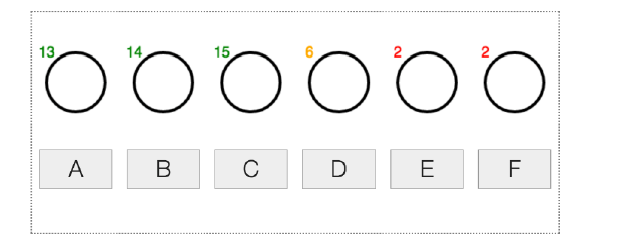
\includegraphics[width=.6\textwidth]{availability.png} \\
\raisebox{1.5cm}{(b)} & 
\includegraphics[width=.55\textwidth]{points.png}
\end{tabular}
\caption{\small{(a) Schematic illustration of the experiment as it appeared to participants in the decreasing availability condition. Each of the six options (A-F) is shown with a colour-coded ``availability counter'', indicating the number of trials left before the option vanishes if left unchosen. The color scheme used red for immediate (1-3), orange for soon (4-6), and green for later (7-15). The display for the constant availability condition removed the availability counters, but was otherwise identical (b) Feedback as it was shown to participants.}}
\label{fig:task}
\end{figure}

The task as described closely mirrors a typical multi-armed bandit task. To introduce option loss into this task, a variant on the game introduced the concept of an ``availability counter'' displayed adjacent to the option. The instructions explained to participants that this counter indicated how long it would be (in terms of number of actions) before this option ``vanished'' if it was not selected. All six availability counters started at a value of 15. The availability counters for every non-selected option would decrease by one after every action, whereas the counter for the selected option would reset to 15. To ensure that the availability counters were visually salient, they were colour-coded: options that were close to vanishing (availability 1-3) were shown in red, options that would disappear soon (availability 4-6) were shown in orange, and other options were shown in green (availability 7-15). Once the availability of an option reached zero it ``expired'': the option and the corresponding response button both disappeared from the screen and could no longer be selected.

In all versions of the task, the rewards $r$ generated by each option were sampled from a normal distribution with mean $\mu$ and fixed standard deviation $\sigma_n = 6$. Two of the six options (randomly chosen) were initially set to have mean reward $\mu = 20$, one had mean $\mu = 40$, one had $\mu = 60$ and the remaining two had $\mu = 80$. However, for most participants the expected value of each option drifted randomly across trials: the mean $\mu_{t+1}$ for any given option on trial $t+1$ was sampled from a normal distribution with centred on the mean from the previous trial $\mu_t$, with variability given by the standard deviation $\sigma_o$ (which differed between conditions).

\subsubsection{Design}

Both experiments employed a 2 x 3 between-subjects design, with the availability of options (\textit{constant} or \textit{diminishing}) and the rate of environmental change (\textit{static}, \textit{slow} and \textit{fast}) as the manipulated variables. For the constant availability condition, options remained available throughout the task, whereas in the diminishing availability condition participants were given the version of the task in which options could vanish, as described above. To create the three levels of environmental change, we set $\sigma_o = 0$ in the static condition, $\sigma_o = 6$ in the slow condition, and $\sigma_o = 12$ in the fast condition.

The two experiments were matched in every detail except one. In Experiment 1, the rewards $r$ were constrained to lie between 1 and 99 points, and a corresponding constraint was placed on the mean $\mu$.\footnote{This was implemented by forcing any values outside the range to lie at the boundary value, producing a slightly "sticky" boundary.} In Experiment 2 the upper bound was removed, allowing the rewards to increase well beyond the initial value. The original motivation for doing so was to see what effect the ceiling has on people strategies, but it quickly became apparent that removing the upper bound can change the dynamics of the task environment. An illustration of what the dynamic structure of the environment looked like for {\it static}, {\it slow} and {\it fast} conditions in both experiments is shown in Figure~\ref{fig:typicaltask}. When the dynamics apply only over a bounded range (Experiment 1) it is quite typical to see the best options change: good options go bad and vice versa. When the bound is removed (Experiment 2) it is quite common to see a ``runaway winner'' where one option quickly dominates over all the others and remains dominant for the entire task. Accordingly, the main goal for pursuing both versions of the task was exploratory, to see how people respond to environments with these different dynamic structures.

\begin{figure}[t]
\centering
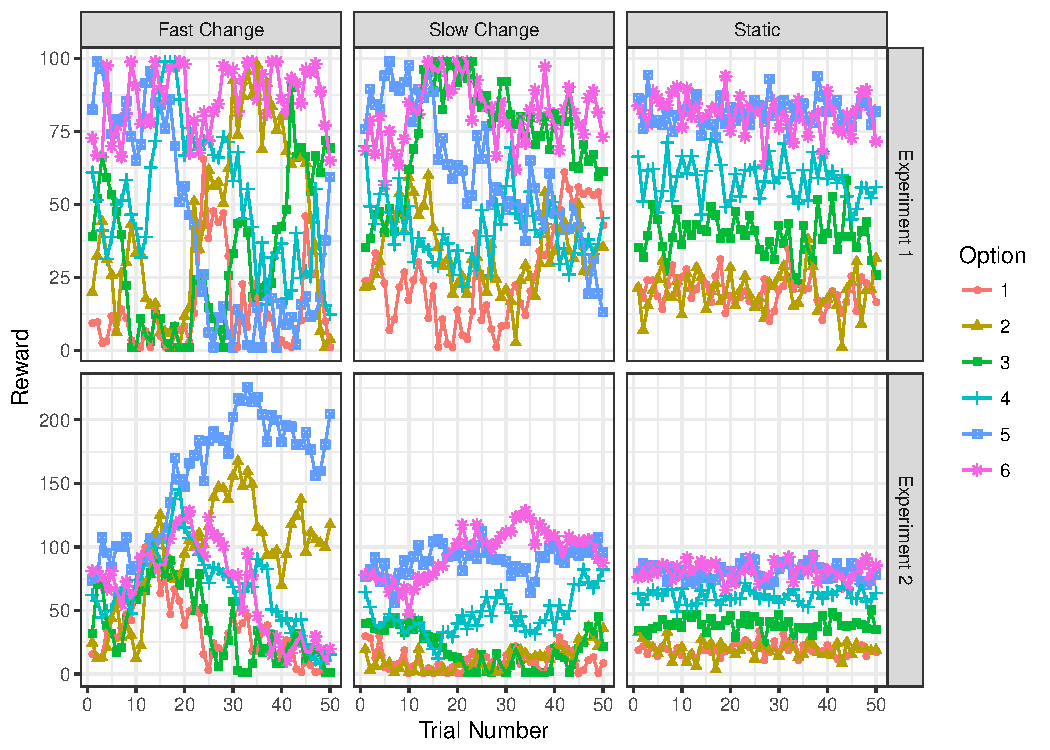
\includegraphics[width=.9\textwidth]{typicaltask.pdf}
\caption{\small{Illustration of the dynamics used in both experiments and all three conditions.}}
\label{fig:typicaltask}
\end{figure}




\subsubsection{Participants}

Workers from Amazon Mechanical Turk were recruited to participate in the experiment (400 in Experiment 1, 300 in Experiment 2), and assigned randomly to conditions. Informed consent was obtained from all participants. As per the exclusion criteria, two participants were excluded from analyses because they selected the same option on every trial. For Experiment 1, 179 participants identified as female, 219 as male, and 2 selected other. Mean reported age was 34.9 (SD = 11.4; range = 18-76). For Experiment 2, 110 participants identified as female, 190 as male. Mean reported age was 34.4 (SD = 10.4; range 18-73). In both experiments participants were almost exclusively ($>$95\%) located in the United States. Tasks took about 10 minutes to complete and participants were paid US\$1.70 for their time.

\subsubsection{Materials and procedure}

Experiments were implemented as a custom web application hosted using Google Cloud Platform, and made available to participants via Amazon Mechanical Turk. At the beginning of the experiment, participants were told they were taking part in a decision-making game as part of a short psychological study investigating how people make decisions. They were then presented with a consent form which informed them about the study and its possible risks; the nature of confidentiality and disclosure of information; and their compensation for completing the task. After providing consent and demographic information, they received instructions corresponding to their assigned condition. To ensure that the participants understood the task, they then had to complete a knowledge check which consisted of three multiple choice questions. Failure to answer all three questions correctly resulted in participants being redirected back to the instructions page to recheck their knowledge before retaking the knowledge check. Participants were then directed to the actual game and completed it as per instructions of the previous page. Following the approach taken in earlier papers \citep{navarro2016learning,HotalingNN_skilledcogsci} each participant played the ``game'' three times (where each game is a 50 trial bandit task), always in the same condition. At the end of each game, participants were told how many points they had achieved, in comparison to the theoretical maximum (and minimum) scores that could be achieved if one were to select the best (or worst) option on every trial. After participants had completed the three games, a completion screen appeared that signalled the  end of the experiment. They were then given a completion code to receive payment through Amazon Mechanical Turk.\footnote{Source code for the experiments is included in the OSF repository along with data and analysis code, but for convenience demonstration versions of the experiment are available at \url{http://compcogscisydney.org/exp/\#vanish}}

\subsection{Results and discussion}


\begin{figure}[t]
\centering
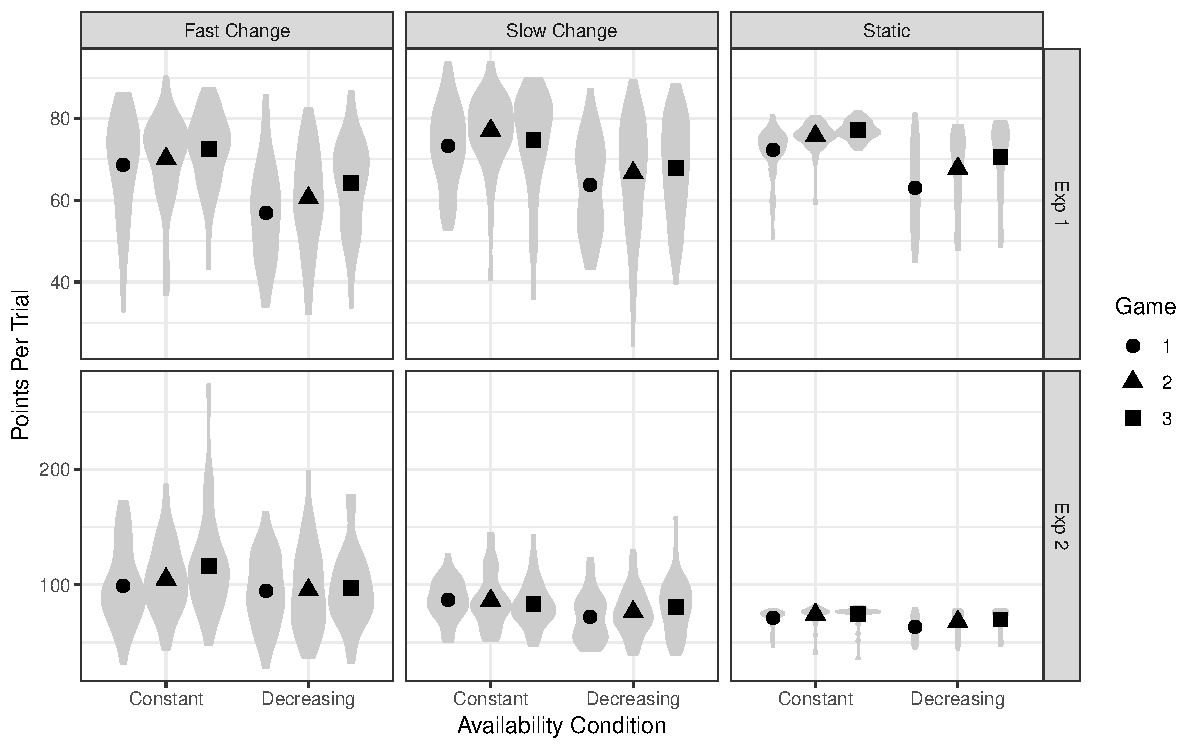
\includegraphics[width=.9\textwidth]{game_points.pdf}
\caption{\small{Average points awarded per action, plotted as a function of game, experiment and condition. Grey violin plots show kernel density estimates of the between subject distribution (averaged over trial), and solid markers show the average across participants.}}
\label{fig:points}
\end{figure}

As a simple measure of performance we calculated the average number of points per action that each participant received during the game. Illustrating this, the solid markers in Figure~\ref{fig:points} plot the mean score per action for every experiment, game, dynamic condition and availability condition; grey violin plots display kernel density estimates of the distribution across  subjects. Although point scores are not easy to compare across conditions or experiments, they are comparable across  games. As shown in Figure~\ref{fig:points} there is a slight tendency for scores to improve over games. In Experiment 1, the mean of points awarded per action rose from 65.5 in game 1 to 70.5 by game 3, with 283 of 400 (71\%) of participants scoring higher on the final game than on the initial one. In Experiment 2, the numbers were 81.0 and 87.2 respectively, with 202 out of 300 (67\%) of participants scoring higher on the final game.
 For simplicity our initial analyses aggregate performance across games, but we return to this topic when introducing model based analyses.

\begin{figure}[t]
\centering
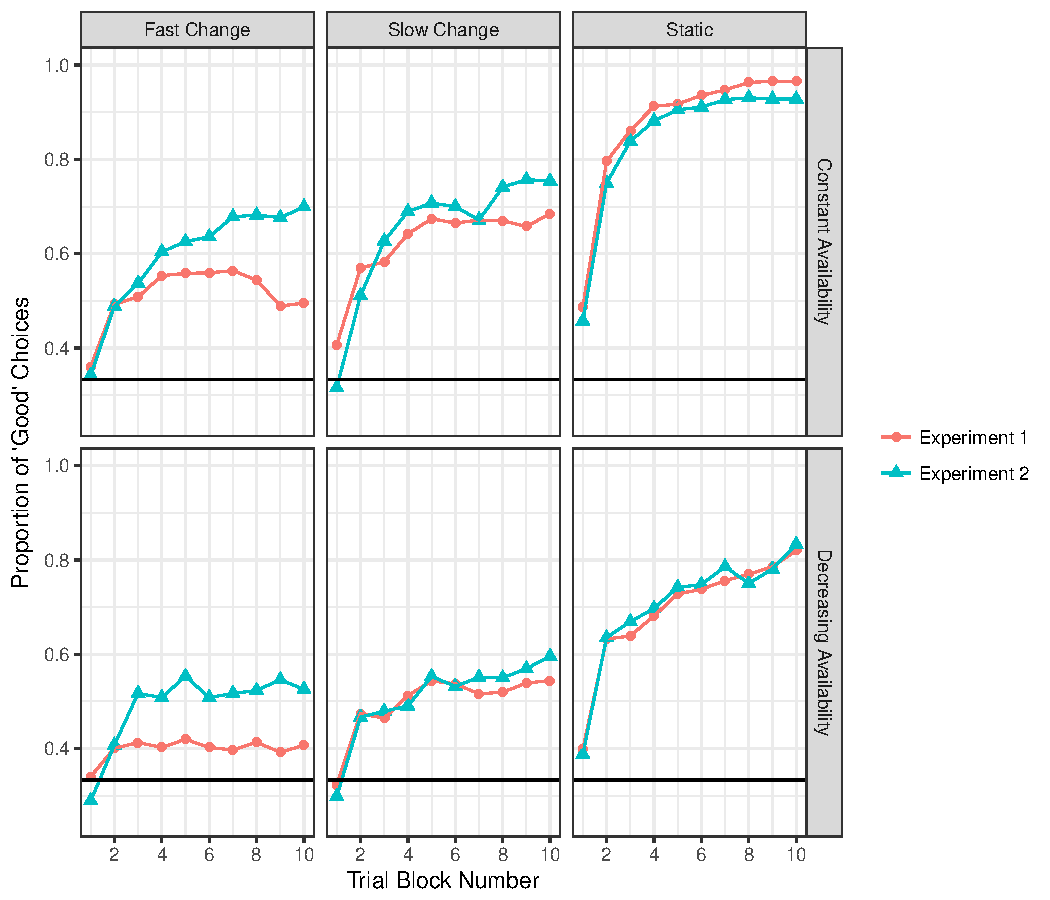
\includegraphics[width=.9\textwidth]{humanperformance.pdf}
\caption{\small{Human performance in the task. Panels plot the probability of choosing a "good" option (one of the top two) on every block of five trials, broken down by experiment, availability and dynamics.}}
\label{fig:goodchoices_human}
\end{figure}

To examine performance at a finer grain, we classified individual responses as a ``good'' choice if it is among the two options with highest expected reward on that trial, including options that have been allowed to expire. Using this measure, the results for all six conditions in both experiments are plotted in Figure~\ref{fig:goodchoices_human}, aggregated across subjects and repeated games, and plotted in blocks of five trials. As is clear from inspection participants learned to make good choices. When the environment was \textit{static} and option availability was \textit{constant}, participants chose good options in the final block on 96\% of cases in Experiment 1 and 93\% in Experiment 2, but when options could vanish in the \textit{decreasing} condition these numbers fell to 82\% and 82\% respectively. The same pattern is observed in the \textit{slowly-changing} restless bandit task, with performance levels of 68\% and 75\% in the \textit{constant availability} conditions in Experiments 1 and 2 falling to 54\% and 60\% in the \textit{decreasing} condition. In the \textit{fast-changing} environment there was a difference between Experiments caused by the fact that the unbounded drift in Experiment 2 allowed for the possibility of a ``runaway winner'' -- where one option grows much faster than all the others as illustrated in the lower left panel of Figure~\ref{fig:typicaltask} --  so final performance in the constant availability was only 50\% in Experiment 1 but 70\% in Experiment 2. Importantly, however, the effect of allowing options to become unviable was the same as in other cases: the performance drops to 41\% and 53\% respectively. In every case a Bayesian t-test found strong evidence for a difference in the proportion of good choices constant availability and decreasing availability (Bayes factors for the alternative, BF$_{10}$, were never less than 47).\footnote{Analyses were conducted using the BayesFactor R package version 0.9.12-2 \citep{morey2015bayesfactor}, using default priors in all cases (i.e., t-test analyses placed Cauchy priors with scale $r=\sqrt{2}/2$ over standardised effect sizes for $H_1$, and ANOVA analyses used JSZ priors with medium scale value $r=1/2$). See \protect\citet{rouder2009bayesian} and \protect\citet{rouder2012default} for specifics. The t-tests reported here used the mean probability of a good choice across all trials as the dependent measure (in order to minimise sensitivity to noise), but the result is robust to the choice of operational measure: the same pattern of results is found if the analyses are conducted looking only at the final trial block.}

\begin{figure}[t]
\centering
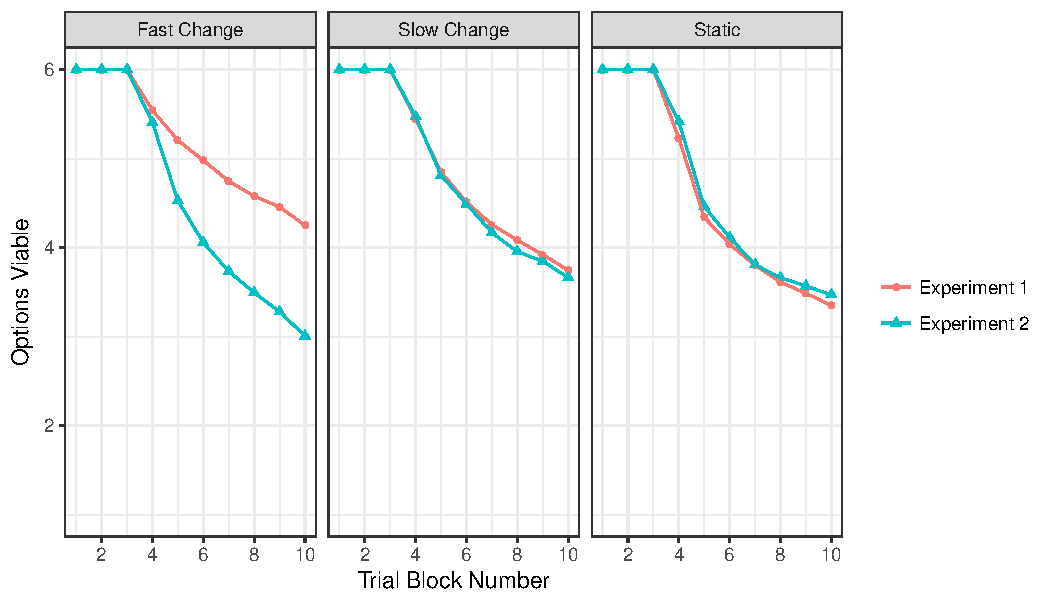
\includegraphics[width=.9\textwidth]{optionsretained.pdf}
\caption{\small{The average number of options still viable in the {\it decreasing availability} condition, plotted separately for the three dynamic conditions, two experiment and for every block of five consecutive trials.}}
\label{fig:optsleft_human}
\end{figure}

To what extent do people keep options alive in the {\it decreasing availability} condition? Figure~\ref{fig:optsleft_human} plots the average number of options still viable as a function of trial block, rate of change, and experiment. Visual inspection of the plot suggests that there are no differences between Experiments 1 and 2 for the \textit{static} and \textit{slow change} conditions (BF$_{01}$ = 4.8 and 5.1 respectively), but in Experiment 2 people retained fewer options in the \textit{fast change} condition than they did in Experiment 1 (BF$_{10}$=89). The latter is perhaps unsurprising in light of the fact that the dynamics of the \textit{fast change} environment in Experiment 2 are rather different from those in Experiment 1, as depicted in Figure~\ref{fig:typicaltask}.

One question of theoretical interest is whether the number of options that remain viable changes as a function of the dynamics of the environment. In Experiment 1, a Bayesian ANOVA suggests there is moderately strong evidence (BF$_{10}$ = 19.1) for the claim that on average people retained slightly more options -- operationally defined as the average number of options still viable, taken across all trials -- as the volatility of the environment increased, rising from 4.6 (SD = 0.9) in the \textit{static} condition to 4.9 (SD = 1.1) in the \textit{slow change} condition and 5.2 (SD = 0.8) in the \textit{fast change} condition. In Experiment 2, however the evidence weakly favoured a null effect (BF$_{01}$ = 6.7): the average number of options retained shows no systematic pattern (mean = 4.7, 4.8 and 4.6 in \textit{static}, \textit{slow} and \textit{fast} respectively; SD = 0.9, 1.1, 1.1).


\subsection{Model based analysis}

The fact that performance declines when option threat is introduced to the task is consistent with previous literature, and is unsurprising. To obtain a more detailed perspective on how people respond to this manipulation, a computational approach is helpful. To minimise researcher degrees of freedom, our approach is derived from the systematic investigation of restless bandit tasks by \cite{speekenbrink2015uncertainty}. Specifically, we relied on the model that provided the best account of the largest number of individual participants in that paper, namely a Kalman filter learning model with a Thompson sampling decision rule. The Kalman filter learning rule provides a Bayesian approach to reinforcement learning \citep{daw2006cortical} that is well-suited to learning in dynamic environments. According the Kalman filter model, the learner's knowledge is represented by a posterior distribution over the expected reward associated with each option\footnote{More generally one might use prospect theory \protect\citep{tversky1992advances} to specify reference-point dependent nonlinear utility functions as \protect\cite{speekenbrink2015uncertainty} did, but in this case a simpler approach where the utility is assumed to be proportional to the number of points received provided a perfectly adequate account of the data, so we avoid introducing this complexity here.}, and under a Thompson sampling decision rule the model selects options with with probability proportional to the chance that they have maximum utility. See Appendix for details.\footnote{It is worth noting that the manner in which we are using the Kalman filter model here is roughly in accordance with what \citep{tauber2017bayesian} refer to as ``descriptive Bayesian modelling". While we do use it as a sensible standard against which we can evaluate human behaviour, we do so because it has a track record of performing well as an empirical model of human reinforcement learning. The fact that it has a meaningful interpretation as a form of probabilistic Bayesian reasoning is an added bonus as it allows us to link model parameters to assumptions about the world. We do not claim that it should be viewed as a genuine normative standard for the task, though we note that in practice human performance rarely surpasses the Kalman filter in our data.}

 To provide a strong test of the Kalman filter model's ability to capture human behaviour on a standard (i.e., constant availability) restless bandit task, we do not estimate any free parameters. Instead, all parameters associated with the noise and volatility in the environment were fixed {\it a priori} at the true values for each condition, and prior distributions were fixed to be very diffuse (see Appendix). Moreover, the model was not yoked to participant responses, and predicted the sequence of responses without being fed information about how human participants responded in the task \citep[e.g.,][]{yechiam2005comparison,steingroever2014absolute}. In all cases, model predictions are averaged across 500 independent simulations.

\subsubsection{Proportion of good choices}



\begin{figure}[t]
\centering
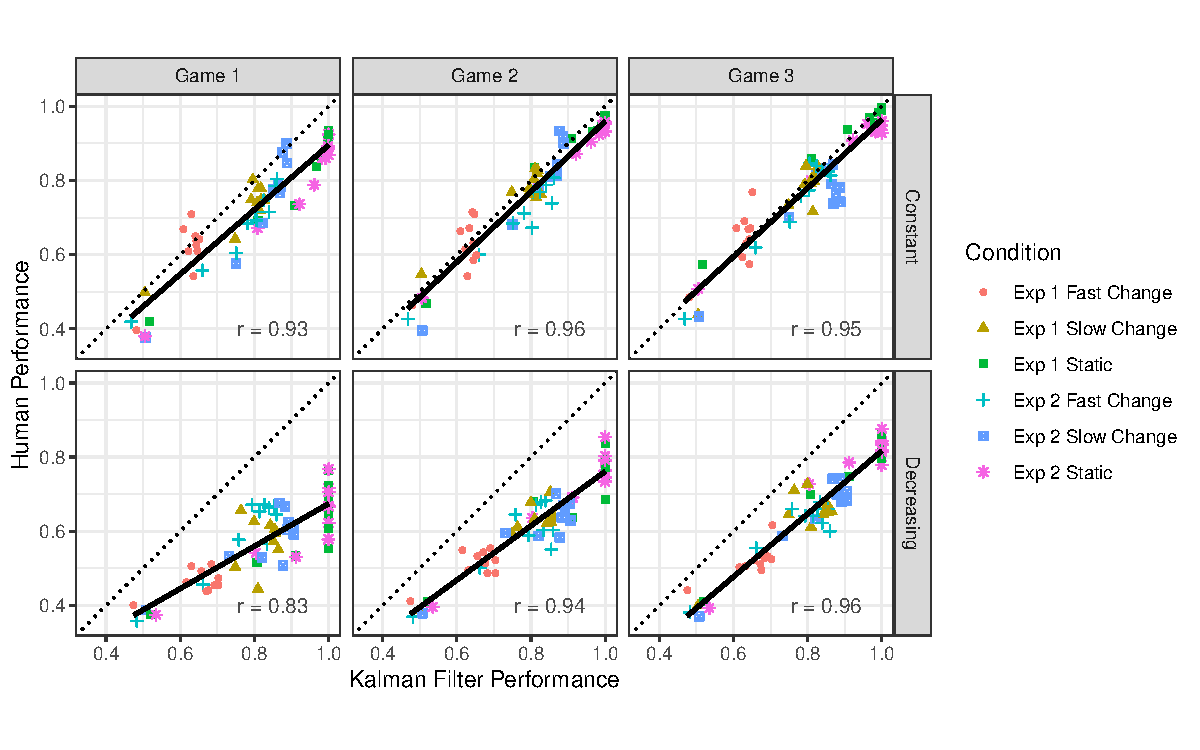
\includegraphics[width=.95\textwidth]{modelvshuman.pdf}
\caption{\small{Human performance versus a Kalman filter model across all conditions and both experiments. The dependent variable plotted in this figure is the probability of making a ``good'' choice (operationally defined as one of the top two options). Each dot represents human and model performance aggregated across subject and across model runs, with each block of five trials, experiment and condition plotted separately. For the human data, the results are plotted separately by game (Kalman filter responses are the same in every game).}}
\label{fig:modelhuman}
\end{figure}

Despite the somewhat stringent nature of the test, the Kalman filter model makes good predictions about human performance in the standard restless bandit task, as shown in the top row of Figure~\ref{fig:modelhuman}. These plots show every data point from the human data in Figure~\ref{fig:goodchoices_human} plotted on the y-axis, broken down by game number, against the corresponding choice probabilities that emerged from the Kalman filter model simulations on the x-axis. Across two experiments, three levels of volatility and ten trial blocks, the correlation between model predictions and human performance ranged from $r=.93$ to $r=.96$ across games. Perhaps more impressively, the best fitting regression line (solid line) is only slightly below the ``perfect'' regression line with slope zero and intercept one (dotted line). In light of this, it is not unreasonable to propose that the decision strategies that human participants applied in the standard restless bandit task are well-approximated by the Kalman filter model.

With this in mind, we can take the Kalman filter model and apply it to the decreasing availability conditions, to obtain some insight into what ``would have'' happened if participants had employed the same strategies in both versions of the task. When we do this we obtain a systematic effect as illustrated in the lower panels of Figure~\ref{fig:modelhuman}. While the model still correlates well with human performance (ranging from $r=.83$ to $r=.96$) the regression line is now substantially shallower, especially for the earlier games. When compared against the Kalman filter model, people were much less likely to select a good option in the vanishing bandit task, despite the fact that in the standard task human performance and the Kalman filter were largely indistinguishable.

\subsubsection{Switching between options}

A slightly different perspective is offered by Figure~\ref{fig:recency}, which plots the proportion of trials on which human participants switched options (i.e., made a different choice than the one made on the previous trial) against the corresponding proportion for the Kalman filter model. Again, the plots are shown separately for both experiments, all three games, all three dynamic conditions and both availability conditions, with separate markers for each block of five consecutive trials. When the environment is {\it static} and option availability is {\it constant} (top right panel), human participants switch between options at essentially the same rate as the Kalman filter throughout the task and across all three games: the plot markers lie close the dashed line in all cases. When volatility and option loss are introduced to the task, people switch between options in a fashion that differs from the model.

Curiously, the two manipulations have different effects.  First consider what happens when volatility is added within a standard (constant availability) restless bandit task. The top row of Figure~\ref{fig:recency} shows that in the {\it slow change} or {\it fast change} conditions  people tended to switch between options slightly {\it less} than the model (i.e., the markers tend to lie below the dashed lines), which might be expected if people underestimate the volatility of the environment. In contrast, consider the effect of adding option loss. Whereas previously people were switching at a similar or reduced rate to the model, in almost every case the plot markers in the bottom row of Figure~\ref{fig:recency} lie above the dashed line, indicating that people now switch {\it more} often than the model. This would be expected if people are engaging in some deliberate strategy to retain options, or are in some respect averse to allowing the availability counter to drop too low.

\begin{figure}[t]
\centering
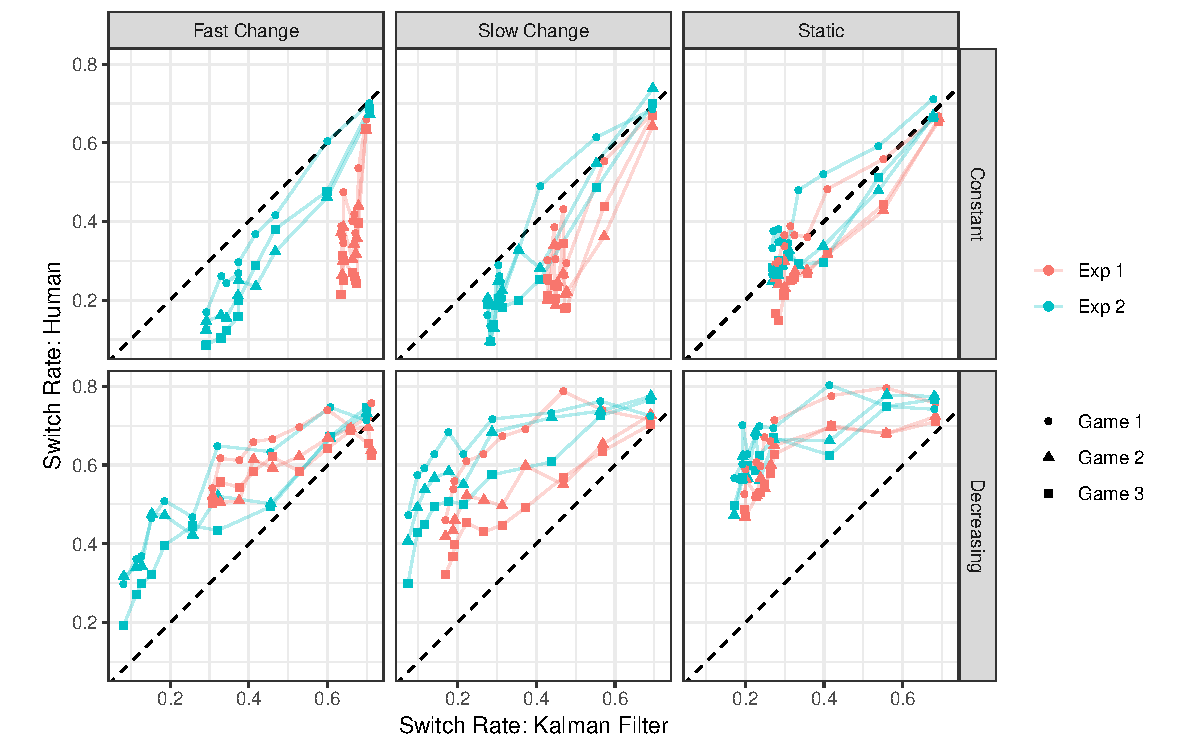
\includegraphics[width=1\textwidth]{recency_comparison_pic.pdf}
\caption{\small{Comparison of the probability of switching options, Kalman filter (x-axis) versus human (y-axis). Every panel displays six plots, one for each experiment and game. Within each plot, individual markers are shown for every block of five trials, with trial block number increasing from right to left. The panels separate the data by availability condition (rows) and dynamic condition (columns). Human participants switch more often than the Kalman filter in the {\it decreasing availability} condition (bottom row), but in the {\it constant} conditions (top row) the switch rates are similar, or show the opposite pattern with humans switching less often.}}
\label{fig:recency}
\end{figure}

\subsubsection{Number of options retained}

\begin{figure}[t]
\centering
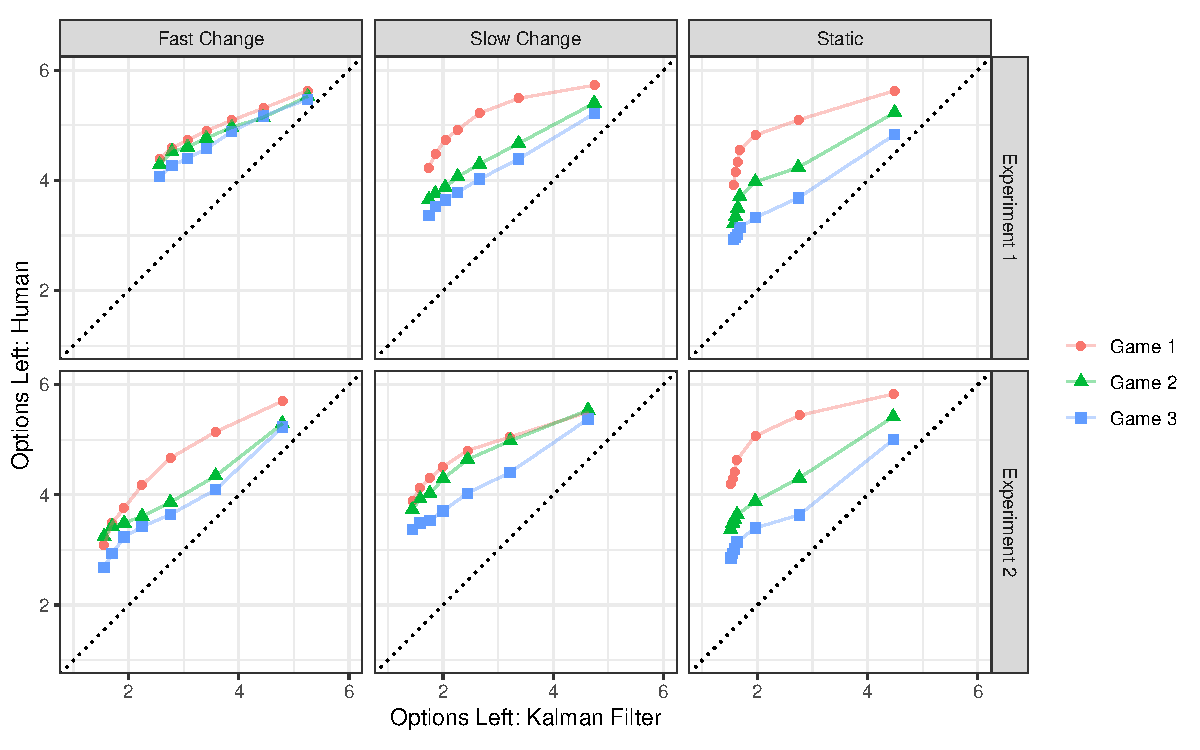
\includegraphics[width=.9\textwidth]{modelvshuman_optleft.pdf}
\caption{\small{Average number of options remaining for human and model in the decreasing availability condition, aggregated across participants and model runs, and plotted separately for trial block, dynamics condition, experiment and game number. Trial block number runs from right to left within each plot.}}
\label{fig:modelhuman_nopts}
\end{figure}

To explore how people adapted to the threat of option loss in more detail, Figure~\ref{fig:modelhuman_nopts} plots the average number of options that remain viable at every stage of the task, for both human participants and the model. As is clear from inspection in every case human participants retained more options than the model: by the end of the task, human participants typically have about 3-4 options still viable, whereas the Kalman filter typically retains only 1-2. Note also that although participants retained fewer options in later games (i.e., in all six panels, the curves shift downward from game 1 to game 3, in no case does the number of options retained fall to the same level as the Kalman filter model. Again this is suggestive of some form of aversion to option loss.


\subsubsection{Choices by availability}

\begin{figure}[t]
\centering
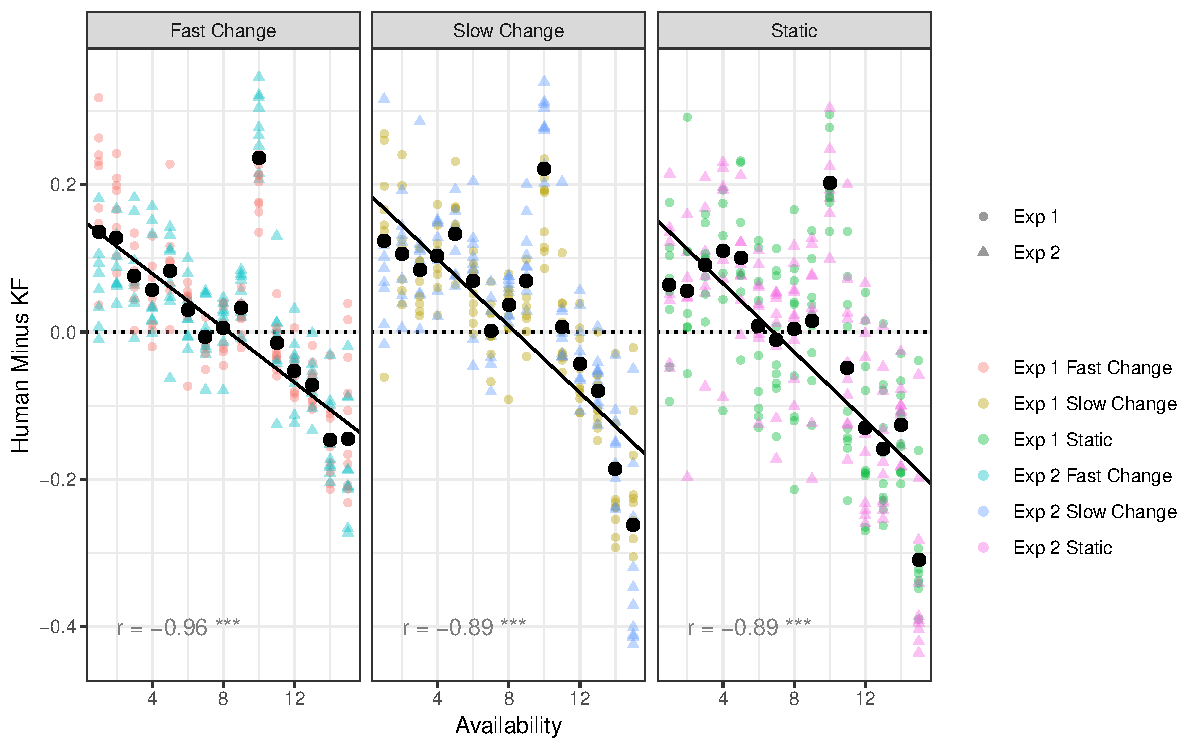
\includegraphics[width=.9\textwidth]{modelvshuman_availdiff.pdf}
\caption{\small{Difference between human and Kalman filter choice probabilities in a vanishing bandit task (y axis), plotted as a function of option availability (x axis) and level of volatility in the environment (panels) and experiment (shape and shading). Averages are plotted as solid black markers, and the regressions (solid black lines) are computed without considering the outlier case at availability 10 (see main text for details). }}
\label{fig:modelhuman_avail}
\end{figure}

If human participants are averse to option loss relative to the Kalman filter model, what precisely is the nature of this difference? Do people roughly follow the Kalman filter model on almost all trials, only occasionally shifting to ``save'' an option on the very last trial before it vanishes? Is the signal driven by perceptual cues, arising only when the option turns red (i.e., when availability drops to three or less)? Or is the effect more continuous, in which the subjective utility associated with choosing an option rises gradually the closer an option gets to vanishing? Although the task was not designed to explicitly test this, we can obtain a preliminary answer computing the average probability of selecting any particular option as a function of its current availability level for both human participants and the Kalman filter model and look at the difference between the two, thereby controlling for the fact that both humans and the model will tend to ignore bad options. If participants are strategically ``saving'' options at the last moment, we should see a spike in human choice probability at availability level 1, whereas if the signal is perceptual this would appear over availability levels 1-3. Alternatively, if a rising urgency explanation is correct, we should see a more gradual bias where humans prefer to choose lower availability options than the model.

The results of this analysis are plotted in Figure~\ref{fig:modelhuman_avail}. With one rather notable exception -- the ``spike'' at availability 10 -- the pattern of results closely mirrors what we might expect if loss aversion takes the form of a gradually rising signal. Across all three levels of volatility there is a smooth, roughly linear relationship between the availability level and the difference score. Visual inspection suggests the possibility that human performance may mirror the Kalman filter model more closely in highly dynamic environments, at least insofar as the correlation appears stronger on the left panel and the slope is flatter, but given the exploratory nature of the analysis this suggestion is somewhat speculative.

Why does the spike at availability 10 occur? The answer is fairly unsurprising but perhaps important. When human participants solve the task, a very typical pattern is to cycle through the options A to F sequentially two or three times, strategically and systematically exploring all six options {\it before} making any decisions about which options are good and which are a bad. If one does this, the decrease in availability means that (with 6 options that reset to availability 15 after they are selected) people will produce a ``run`` of choices at availability 10 during the exploratory phase. The Kalman filter model has no equivalent behaviour. Because the model  does not encode motor costs associated with switching (why jump from option A to option D when option B is closer?) and does not have any structured encoding of the task that would suggest that an ``initial sweep'' through the options would be a sensible exploratory strategy, it produces no such pattern. From the perspective of understanding aversion to option loss, the observed spike at 10 is somewhat uninteresting, but the strategic nature of the human behaviour that produces it is arguably of considerable interest for thinking about how people solve explore-exploit problems more generally.

\section{General Discussion}

Consistent with previous literature, human performance in short-horizon restless bandit tasks is captured remarkably well with a Kalman filter learning rule and Thompson sampling decision procedure \citep{speekenbrink2015uncertainty}. Even without parameter estimation and making purely {\it a priori} model predictions, the correlation is very strong. When we introduce the threat of option loss to this task, there are systematic departures. While the  correlation between the Kalman filter model and human data remains extremely strong there is a systematic shift in the regression line relating the model and human behaviour. Relative to this model, people retain more options and make less-rewarding choices.

These findings are consistent with the existing literature on option loss \citep{shin2004keeping, bonney2016investigations, ejova2009walk, neth2014foraging}, but provide a stronger test of the claim. The simple fact that options {\it can} vanish in a vanishing bandit task means that two agents following the same underlying strategy might produce vastly different responses -- by using the Kalman filter model as the basis for comparing the two conditions we can control for systematic differences in the structure of the task. Indeed, it is notable that the Kalman filter model also performs worse in the vanishing conditions than it does in the constant availability conditions even though (by design) it makes responses using precisely the same learning and decision rules in both cases. Even so, people's choices in the vanishing conditions tend to be poorer than those of the Kalman filter model, strongly suggesting that people employ different strategies when option loss is present.

\subsection{Explaining the effect of option threat}

Why do people perform worse than the Kalman filter model in the decreasing availability conditions? The results seem intuitively plausible when viewed as a form of loss aversion, but there are other possibilities that should be considered. For instance, one possibility is that these tasks involve a form of ``choice overload''. Having too many options can be overwhelming or demotivating \citep{iyengar2000choice}, and in a multi-armed bandit task, maintaining representations of six possibly volatile reward distributions is likely demanding and people need to trim down the options to something manageable. Though intuitively appealing in one sense -- anecdotally, it does feel cognitively demanding to maintain representations of the values of six entities in working memory while doing this task -- it is unclear why an explanation based on cognitive load would apply only when option viability is threatened.

Another possibility is the idea that people do not plan very effectively in the task. Other work on multi-armed bandit tasks has argued that people are {\it myopic} planners \citep{zhang2013forgetful} who do not look ahead very far when considering their next action. Taken literally, however, a myopic planner should allow options to expire extremely readily, especially when the environment is not too volatile. After all, an option that is currently quite poor is extremely unlikely to suddenly become better in the near future, and it would only be worthwhile retaining it if one's planning horizon were quite {\it long}. An alternative explanation, however, might acknowledge the possibility that people are aware of the limitations in their planning: that is, a ``loss averse'' strategy of retaining more options than one can {\it foresee} a use for might be viewed as a sensible hedge against computational limitations. If I know that my true planning horizon needs to be quite long but I am computationally limited, what should I do? Keeping one's options open, even if one is not quite sure {\it why} could be a very wise strategy, and is somewhat reminiscent of boundedly rational models of wishful thinking \citep{neuman2014bounded} and heuristic models of planning in machine learning \citep{szita2008many}. Indeed, to the extent that knowing when to allow an option to expire has an element of ``predicting one's own future preferences'' to it, it is very likely to be a difficult problem to solve \citep{loewenstein1997predicting} and one that might induce a certain amount of conservatism. Arguably this is not inconsistent with a loss aversion explanation, insofar as loss aversion might be viewed as a sensible adaptation in light of these computational limitations.

To the extent that the results do reflect loss aversion, it is worth thinking about the connection between aversion to {\it option loss} as it is formalised here and in related papers \citep{shin2004keeping,ejova2009walk} and how loss aversion is more typically operationalised in restless bandit tasks. In \citet{speekenbrink2015uncertainty}, for instance, a prospect theory approach based on \citet{tversky1992advances} was used as a mechanism for capturing the aversion to losing some abstracted notion of reward associated with a choice -- points, or monetary rewards -- whereas in vanishing bandit tasks the losses operate at the level of entire {\it options}. If each option in a task is perceived as an affordance (mechanism for future actions in the environment), it seems plausible to think that the subjective feeling of loss aversion in this task is likely to be much stronger than in a typical restless bandit task. Indeed, the experimental design is somewhat reminiscent of tasks studying the endowment effect \citep{kahneman1990experimental}. At the beginning of the task participants are ``given'' six labelled options: in one condition (constant availability) these options are presented as fixed and enduring characteristics of the world, and under these circumstances people value them ``appropriately'', at least in the sense of closely mirroring the pattern of behaviour shown by the Bayesian Kalman filter model. In another condition (decreasing availability) the options available to participants can be ``taken away'' by the experiment(er). It seems plausible that people feel a stronger sense of possession or entitlement to the affordances linked to response options than they do to more any abstract notion of points or even to modest amounts of money, producing a rather large and systematic deviation from the Kalman filter as typically implemented.

\subsection{Towards a computational account}

Although the current work is limited in terms of the variety of modelling approaches we have considered, exploring the space of possible models is a natural direction to extend this work in the future. In this respect, our empirical data provide a number of hints. The (mostly) smooth pattern of deviation shown in Figure~\ref{fig:modelhuman_avail} suggests that the value of returning to a diminishing option {\it gradually} increases with proximity to the disappearance. The one departure from that pattern (the spike at 10) is interesting in and of itself, as it strongly suggests a {\it systematic} exploratory strategy during the early stages of the task \citep[see][]{acuna2010structure}. Nevertheless, with the exception of this one systematic exploratory strategy, it does not seem technically difficult to capture the pattern of behaviour within the Kalman filter framework.

The simplest possibility would be to suggest that different Kalman filter parameter values apply when option threat is present. For instance, when options can vanish people might act as though the world is more volatile than they otherwise would (e.g., increase the parameter $\sigma_w$ that governs beliefs about the rate of change in reward rates). This would lead to increased exploration of alternatives, which in turn would ensure that fewer options disappear. Alternatively, one could capture the effect by modifying the reward function: the subjectively experienced reward $r_t$ associated with choosing an option might depend not only on the number of ``actual'' points received, but also upon the effect that the choice has on availability. That is, selecting an option that is about to expire might be {\it inherently} rewarding because of the gain to the availability total.

Looking beyond the Kalman filter, one possibility is to use dynamic programming to work out the optimal decision policy for the task under a variety of different assumptions \citep[e.g.,][]{littman2009tutorial}. For example, if people believe that the reward rates are more volatile than it is (or the horizon for the task is longer than the 50 trials than it really is), a rational strategy would be to ``cling'' to more options than are really needed. This would produce sub-optimal behaviour in the {\it task} purely as a consequence of misconstruing the nature of the problem. Another alternative is to consider heuristic models. In option loss problems, after an initial exploratory sweep through the options, people might alternate between exploitation phases (always select the best option) and  exploration phases (preserve/try all options). This two-mode strategy would be relatively simple to implement and could potentially describe performance in a variety of problems.

Finally, the fact that human performance improves across games provides an avenue for future modelling. The approach that we have taken in this paper is to give people a series of short sequential decision making tasks, and consistent with our earlier work adopting this approach \citep{navarro2016learning,HotalingNN_skilledcogsci} there is a small but consistent effect. In future work we hope to investigate up a wider range of these transfer effects in order to develop computational models that describe the higher order learning that people do within sequential decision tasks.

\subsection{How is option threat interpreted?}

Regardless of what formal account best captures human behaviour in the task, it seems there is another puzzle: {\it why} does the signal scale in the linear fashion shown in Figure~\ref{fig:modelhuman_avail}? In the task as currently operationalised, an option that has availability level 11 is no more likely to vanish in the short term than an option with availability level 15. At these levels, the ``threat'' of vanishing is so distant that it ought not to have any substantial effect on people's behaviour even if they {\it are} averse to option loss -- after all, with a maximum of 6 options in the task, it would be possible for the decision maker to revisit  every other response option {\it twice} without any risk of losing an option with availability 11. Realistically, it does not seem plausible to think that this task incorporates any meaningful difference in ``threat'' between availability levels 11 and 15. Nevertheless, the data do  suggest that people treat these cases differently in the vanishing bandit task. Despite the fact that the availability counter merely expressed the known length of time before any losses would be incurred, and does not reflect any probability of immediate loss, people responded to the counter as if it represented something more akin to an increased {\it hazard}.

The reasons for this are not immediately apparent. In real life, of course, there are many situations in which proximity to a threat does imply increased hazard, and so it might be the case that people are simply over-generalizing from those situations. Sometimes proximity to a danger can increase the {\it magnitude} of the associated losses (e.g., being closer to a heat source increases the amount of burning), and at other times it affects {\it probability} of incurring a loss (e.g., the closer to a predator one gets the greater the likelihood of an adverse event). While this does sound plausible, it is also the case that there are other scenarios that do not work this way. For instance, except at very close distances, approaching the edge of a cliff does not increase the risk of falling off. The structure of the vanishing bandit task has more in common with ``falling off a cliff'' than it does with ``being eaten by a tiger'', yet people treat it more like the latter. It is not immediately obvious -- to us at least -- why falling off a cliff represents less of an ecologically plausible risk than being eaten by a tiger, so it is not clear why people appear to interpret the availability counter as if it reflected a rising hazard. This seems a worthwhile direction for further work.

\bibliography{vanishing}

\section{Appendix}

The Kalman filter provides a Bayesian reinforcement learning model that assumes the utility of options across time follows a Gaussian process, and as such is fairly well matched to the structure of the task. Our implementation of the Kalman filter model is taken from \citet{speekenbrink2015uncertainty}, with one simplification: we assume that the utility $u_t$ of the reward $r_t$ received on trial $t$ is simply  $u_t = r_t$, and do not fit a subjective prospect curve. The Kalman filter estimate of the expected utility $E_{jt}$ of option $j$ on trial $t$ is calculated via a simple update rule:
$$
E_{jt} = E_{j,t-1} + \delta_{jt} K_{jt} \left( r_t - E_{j,t-1} \right)
$$
where $E_{j,t-1}$ is the estimate of the expected utility from the previous trial, $\delta_{jt}$ is an indicator function that equals 1 if arm $j$ was chosen on trial $t$ and 0 otherwise, and $K_{jt}$ describes the {\it Kalman gain},
$$
K_{jt} = \frac{S_{j,t-1} + {\sigma_w}^2}{S_{j,t-1} + {\sigma_n}^2 +  {\sigma_w}^2}
$$
In this expression $\sigma_n$ is the learners belief about the standard deviation of the noise and $\sigma_w$ is their belief about the rate of change in the underlying stochastic process. For our examples we fix these at their true (ideal observer) values, yielding $\sigma_n = 6$ for all conditions, and a value of $\sigma_w$ that depends on the environment volatility: 0 in the static condition, 6 in the slow condition and 12 in fast condition. The value of $S_{jt}$ is the variance of the posterior distribution (after trial $t$) over the mean utility associated with option $j$ and is given by
$$
S_{jt} = (1-\delta_{jt} K_{jt})(S_{j,t-1} + {\sigma_w}^2)
$$
We set prior means and variances to  $E_{j0} = 50$ and $S_{j0} = 1000$ respectively.

The decision rule we used is a variation of the Thompson sampling rule, also known as probability of maximum utility, PMU. For option $j$ on trial $t$, the learner's posterior belief about the mean reward associated with that distribution is Gaussian with mean $E_{jt}$ and standard deviation $S_{jt}$. We assume a stochastic decision rule where the perceived value of this option $v_{jt}$ is represented by a single draw from this posterior \citep{vul2014one}, and the decision maker always chooses the option with maximum perceived value (i.e., $\arg \max_j v_{jt}$). In some versions of the Thompson sampling rule one samples proportional to the (posterior predictive) probability that the option will yield the highest {\it actual} reward $r_t$ on trial $t$, whereas another variation might sample proportional to the posterior probability that an option has the highest {\it expected} reward $\mu_t$ on that trial. The latter version is implemented here.


\end{document}

